%%%%%%%%%%%%%%%%%%%%%%%%%%%%%%%%%%%%%%%%%%%%%%%%%%%%%%%%%%%%%%%%%5
\section{Reconstructions}
\label{s:appendix-reonstructions}


\section{P-value analysis}
\label{s:appendix-pvalue}

Four p-value analyses have been performed, one for each autoencoder model (convolutional and recurrent) in the short-term and very short-term settings.

\newpage

\begin{figure}[!h]
    \centering
    \begin{minipage}{0.5\textwidth}
        \centering
        \includesvg[width=\linewidth]{figures/experiments/p_val/model_0_ts.svg}
    \end{minipage}%
    \begin{minipage}{0.5\textwidth}
       \centering
       \includesvg[width=\linewidth]{figures/experiments/p_val/model_0_pvalues.svg}
    \end{minipage}
    \captionsetup{width=0.9\linewidth}
    \caption{TS distribution and p-values for the autoencoder with convolutional layers in the short-term scenario (integration time = 5 seconds).}
    \label{fig:ts-distribution-and-p-values-cnn-it-5-appendix}
\end{figure}

\begin{table}[!h]
\centering
\begin{tabular}{|p{3cm}|p{3cm}|p{3cm}|p{3cm}|}
\hline
\multicolumn{4}{|c|}{p-values} \\
\hline
Threshold & p-value & $\pm$ error &  Sigma \\
\hline
0.003171 & 1.283972e-01 & 1.201785e-04 & 1.134 \\
0.003751 & 6.115264e-02 & 8.293861e-05 & 1.545 \\
0.004476 & 2.277199e-02 & 5.061155e-05 & 2.000 \\
0.005492 & 5.323285e-03 & 2.447028e-05 & 2.554 \\
0.006507 & 1.228234e-03 & 1.175411e-05 & 3.029 \\
0.007667 & 2.312711e-04 & 5.100465e-06 & 3.502 \\
0.009118 & 3.149606e-05 & 1.882250e-06 & 4.001 \\
0.010859 & 3.262092e-06 & 6.057553e-07 & 4.509 \\
0.013905 & 2.249719e-07 & 1.590791e-07 & 5.047 \\
\hline
\end{tabular}
\caption{An example of p-value analysis for the autoencoder with convolutional layers in the short-term scenario (integration time = 5 seconds). The table shows a subset of all the rows. Only the threshold values corresponding to predefined sigma levels are shown.}
\label{tab:p-value-table-cnn-itime-5-appendix}
\end{table}




\begin{figure}[!h]
    \centering
    \begin{minipage}{0.5\textwidth}
        \centering
        \includesvg[width=\linewidth]{figures/experiments/p_val/model_1_ts.svg}
    \end{minipage}%
    \begin{minipage}{0.5\textwidth}
       \centering
       \includesvg[width=\linewidth]{figures/experiments/p_val/model_1_pvalues.svg}
    \end{minipage}
    \captionsetup{width=0.9\linewidth}
    \caption{TS distribution and p-values for the autoencoder with recurrent layers in the short-term scenario (integration time = 5 seconds).}
    \label{fig:ts-distribution-and-p-values-rnn-it-5-appendix}
\end{figure}

\begin{table}[!h]
\centering
\begin{tabular}{|p{3cm}|p{3cm}|p{3cm}|p{3cm}|}
\hline
\multicolumn{4}{|c|}{p-values} \\
\hline
Threshold & p-value & $\pm$ error &  Sigma \\
\hline
0.000227 & 1.416930e-01 & 1.254772e-04 & 1.073 \\
0.000279 & 6.802256e-02 & 8.693953e-05 & 1.491 \\
0.000357 & 2.249792e-02 & 4.999907e-05 & 2.005 \\
0.000462 & 5.975999e-03 & 2.576891e-05 & 2.514 \\
0.000592 & 1.323296e-03 & 1.212605e-05 & 3.006 \\
0.000749 & 2.503472e-04 & 5.274268e-06 & 3.480 \\
0.001009 & 3.077949e-05 & 1.849360e-06 & 4.007 \\
0.001296 & 3.222401e-06 & 5.983849e-07 & 4.511 \\
0.002078 & 2.222346e-07 & 1.571436e-07 & 5.049 \\
\hline
\end{tabular}
\caption{An example of p-value analysis for the autoencoder with recurrent layers in the short-term scenario (integration time = 5 seconds). The table shows a subset of all the rows. Only the threshold values corresponding to predefined sigma levels are shown.}
\label{tab:p-value-table-rnn-itime-5-appendix}
\end{table}

\begin{figure}[!h]
    \centering
    \begin{minipage}{0.5\textwidth}
        \centering
        \includesvg[width=\linewidth]{figures/experiments/p_val/model_6_ts.svg}
    \end{minipage}%
    \begin{minipage}{0.5\textwidth}
       \centering
       \includesvg[width=\linewidth]{figures/experiments/p_val/model_6_pvalues.svg}
    \end{minipage}
    \captionsetup{width=0.9\linewidth}
    \caption{TS distribution and p-values for the autoencoder with convolutional layers in the very short-term scenario (integration time = 1 second).}
    \label{fig:ts-distribution-and-p-values-cnn-it-1-appendix}
\end{figure}

\begin{table}[!h]
\centering
\begin{tabular}{|p{3cm}|p{3cm}|p{3cm}|p{3cm}|}
\hline
\multicolumn{4}{|c|}{p-values} \\
\hline
Threshold & p-value & $\pm$ error &  Sigma \\
\hline
  0.002693 & 1.024839e-01 & 1.067133e-04 &  1.268 \\
  0.003101 & 6.951853e-02 & 8.789033e-05 &  1.479 \\
  0.004732 & 1.846536e-02 & 4.529703e-05 &  2.087 \\
  0.006363 & 5.940219e-03 & 2.569165e-05 &  2.516 \\
  0.009218 & 1.251736e-03 & 1.179362e-05 &  3.023 \\
  0.013295 & 2.115673e-04 & 4.848586e-06 &  3.525 \\
  0.018597 & 2.966831e-05 & 1.815671e-06 &  4.015 \\
  0.025529 & 2.777932e-06 & 5.555864e-07 &  4.543 \\
  0.031646 & 2.222346e-07 & 1.571436e-07 &  5.049 \\
\hline
\end{tabular}
\caption{An example of p-value analysis for the autoencoder with convolutional layers in the very short-term scenario (integration time = 1 second). The table shows a subset of all the rows. Only the threshold values corresponding to predefined sigma levels are shown.}
\label{tab:p-value-table-cnn-itime-1-appendix}
\end{table}

\begin{figure}[!h]
    \centering
    \begin{minipage}{0.5\textwidth}
        \centering
        \includesvg[width=\linewidth]{figures/experiments/p_val/model_7_ts.svg}
    \end{minipage}%
    \begin{minipage}{0.5\textwidth}
       \centering
       \includesvg[width=\linewidth]{figures/experiments/p_val/model_7_pvalues.svg}
    \end{minipage}
    \captionsetup{width=0.9\linewidth}
    \caption{TS distribution and p-values for the autoencoder with recurrent layers in the very short-term scenario (integration time = 1 second).}
    \label{fig:ts-distribution-and-p-values-rnn-it-1-appendix}
\end{figure}

\begin{table}[!h]
\centering
\begin{tabular}{|p{3cm}|p{3cm}|p{3cm}|p{3cm}|}
\hline
\multicolumn{4}{|c|}{p-values} \\
\hline
Threshold & p-value & $\pm$ error &  Sigma \\
\hline
  0.000201 & 1.339528e-01 & 1.245178e-04 &  1.108 \\
  0.000261 & 5.839725e-02 & 8.221515e-05 &  1.568 \\
  0.000322 & 2.368679e-02 & 5.236110e-05 &  1.983 \\
  0.000443 & 6.268881e-03 & 2.693709e-05 &  2.497 \\
  0.000806 & 1.322414e-03 & 1.237199e-05 &  3.006 \\
  0.001018 & 2.312634e-04 & 5.173794e-06 &  3.502 \\
  0.001260 & 3.021008e-05 & 1.869957e-06 &  4.011 \\
  0.002168 & 3.356676e-06 & 6.233190e-07 &  4.503 \\
  0.002623 & 2.314949e-07 & 1.636916e-07 &  5.041 \\
\hline
\end{tabular}
\caption{An example of p-value analysis for the autoencoder with recurrent layers in the very short-term scenario (integration time = 1 second). The table shows a subset of all the rows. Only the threshold values corresponding to predefined sigma levels are shown.}
\label{tab:p-value-table-rnn-itime-1-appendix}
\end{table}



\section{Detection plots}
\label{s:appendix-c}

\begin{figure}[!htb]
    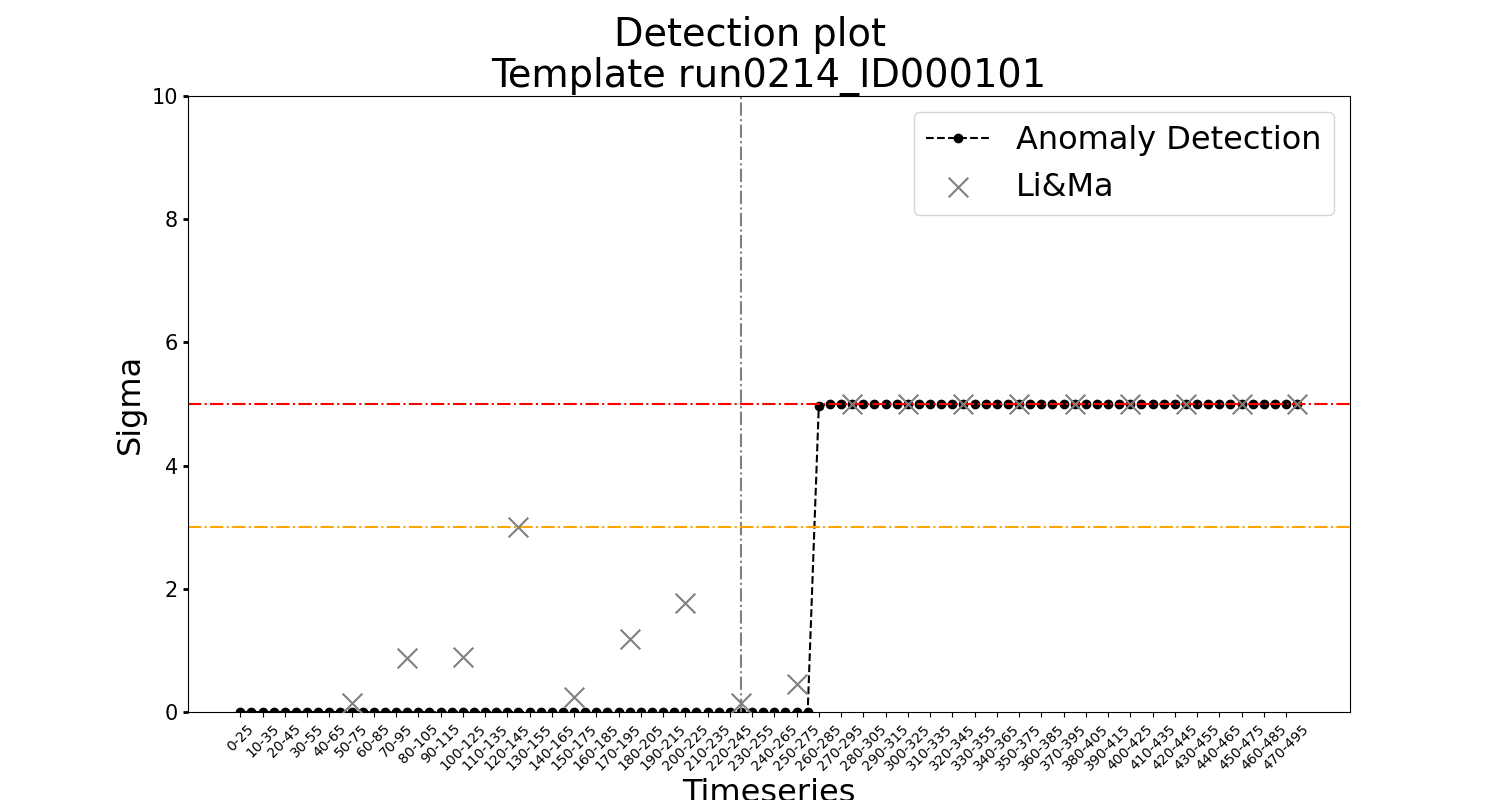
\includegraphics[width=1\textwidth]{figures/experiments/detection_plots/detection_plot_run0214_ID000101_testset_e.png}
\end{figure}
    
\begin{figure}[!htb]    
    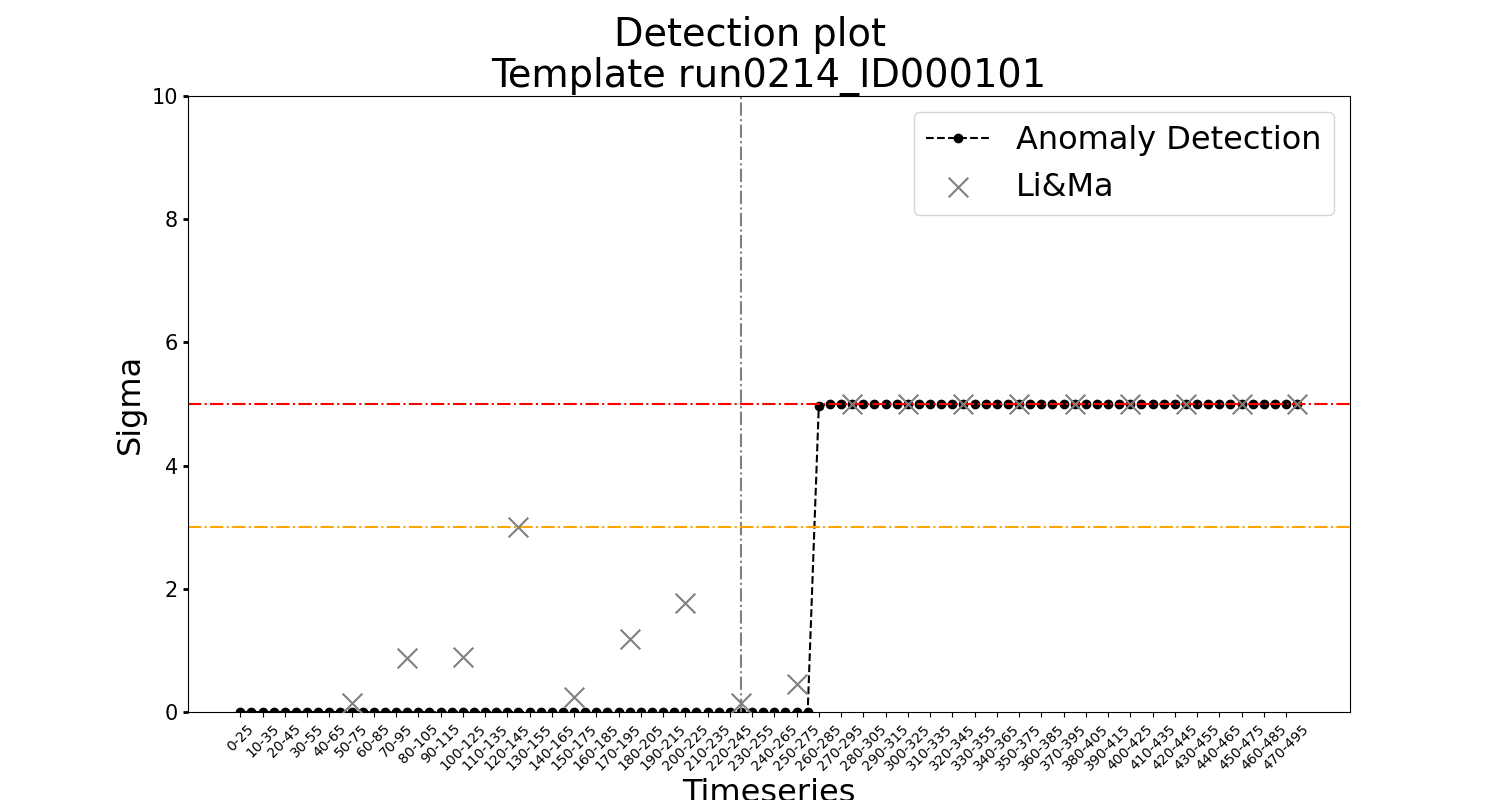
\includegraphics[width=1\textwidth]{figures/experiments/detection_plots/detection_plot_run0214_ID000101_testset_e.png}
\end{figure}
    
\begin{figure}[!htb]
    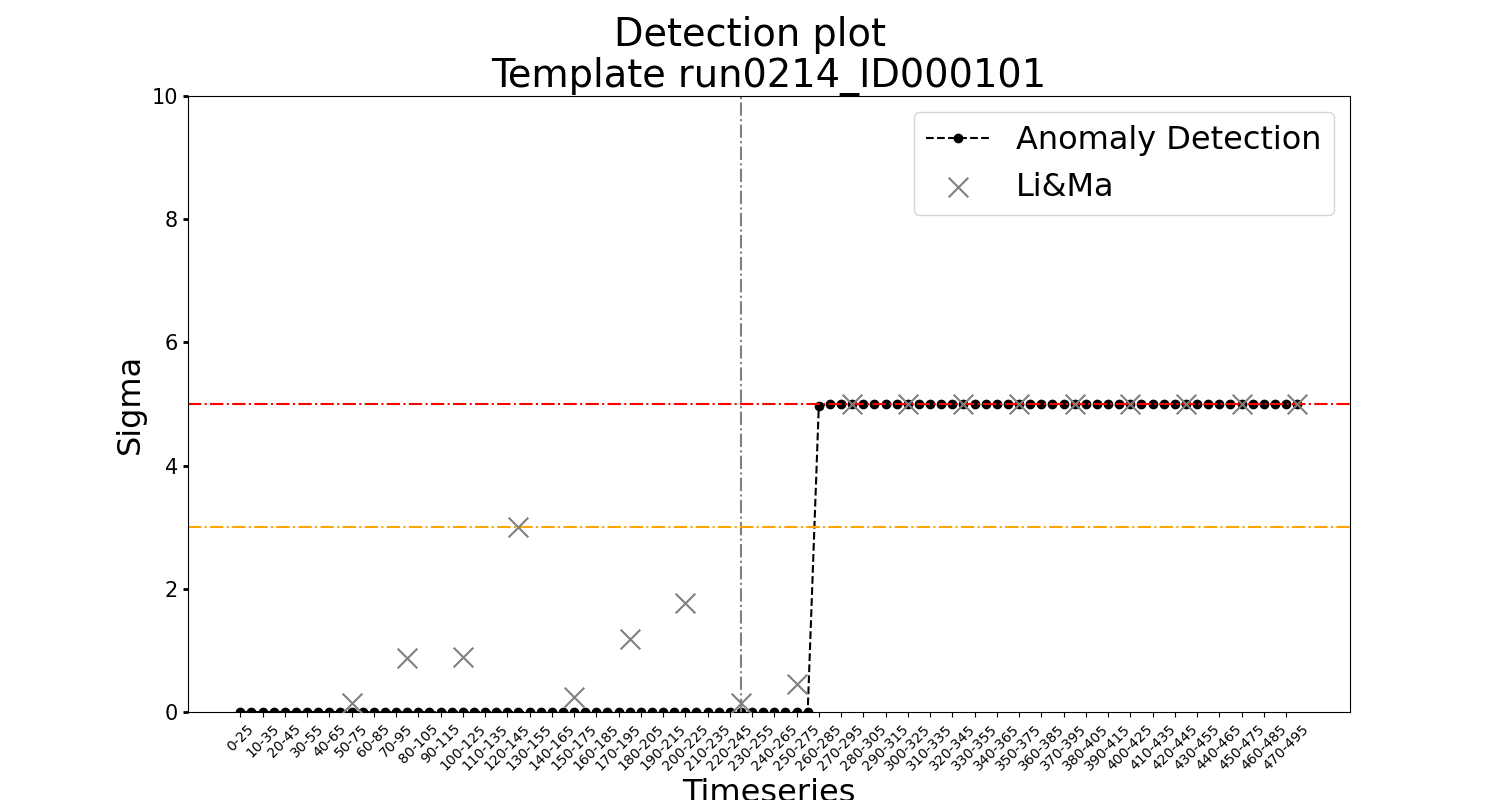
\includegraphics[width=1\textwidth]{figures/experiments/detection_plots/detection_plot_run0214_ID000101_testset_e.png}
\end{figure}

\begin{figure}[!htb]
    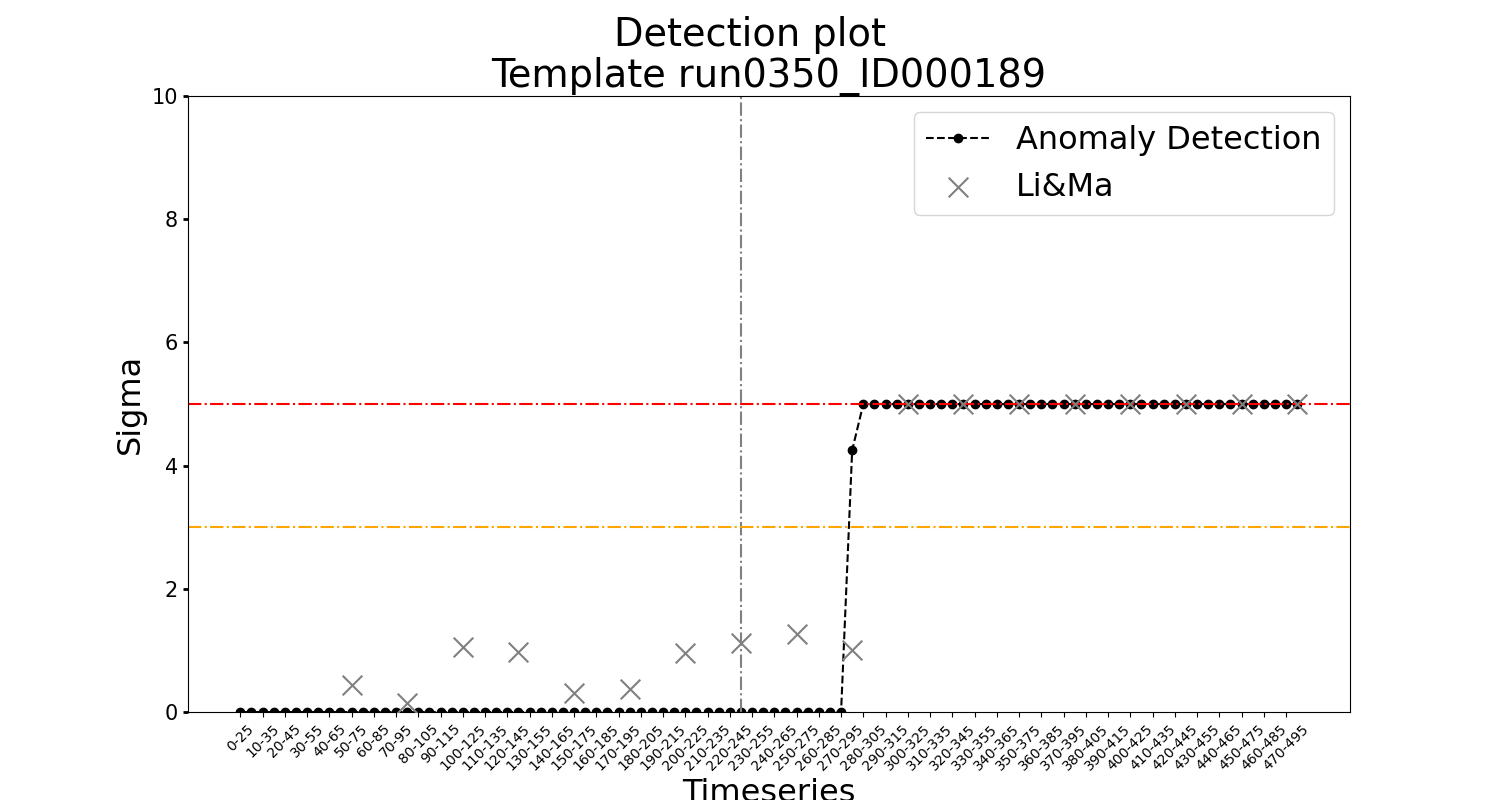
\includegraphics[width=1\textwidth]{figures/experiments/detection_plots/detection_plot_run0350_ID000189_testset_e.png}
\end{figure}

